\documentclass[10pt]{article} % For LaTeX2e
\usepackage{tmlr}
% If accepted, instead use the following line for the camera-ready submission:
%\usepackage[accepted]{tmlr}
% To de-anonymize and remove mentions to TMLR (for example for posting to preprint servers), instead use the following:
%\usepackage[preprint]{tmlr}

% Optional math commands from https://github.com/goodfeli/dlbook_notation.
%%%%% NEW MATH DEFINITIONS %%%%%

\usepackage{amsmath,amsfonts,bm}

% Mark sections of captions for referring to divisions of figures
\newcommand{\figleft}{{\em (Left)}}
\newcommand{\figcenter}{{\em (Center)}}
\newcommand{\figright}{{\em (Right)}}
\newcommand{\figtop}{{\em (Top)}}
\newcommand{\figbottom}{{\em (Bottom)}}
\newcommand{\captiona}{{\em (a)}}
\newcommand{\captionb}{{\em (b)}}
\newcommand{\captionc}{{\em (c)}}
\newcommand{\captiond}{{\em (d)}}

% Highlight a newly defined term
\newcommand{\newterm}[1]{{\bf #1}}


% Figure reference, lower-case.
\def\figref#1{figure~\ref{#1}}
% Figure reference, capital. For start of sentence
\def\Figref#1{Figure~\ref{#1}}
\def\twofigref#1#2{figures \ref{#1} and \ref{#2}}
\def\quadfigref#1#2#3#4{figures \ref{#1}, \ref{#2}, \ref{#3} and \ref{#4}}
% Section reference, lower-case.
\def\secref#1{section~\ref{#1}}
% Section reference, capital.
\def\Secref#1{Section~\ref{#1}}
% Reference to two sections.
\def\twosecrefs#1#2{sections \ref{#1} and \ref{#2}}
% Reference to three sections.
\def\secrefs#1#2#3{sections \ref{#1}, \ref{#2} and \ref{#3}}
% Reference to an equation, lower-case.
\def\eqref#1{equation~\ref{#1}}
% Reference to an equation, upper case
\def\Eqref#1{Equation~\ref{#1}}
% A raw reference to an equation---avoid using if possible
\def\plaineqref#1{\ref{#1}}
% Reference to a chapter, lower-case.
\def\chapref#1{chapter~\ref{#1}}
% Reference to an equation, upper case.
\def\Chapref#1{Chapter~\ref{#1}}
% Reference to a range of chapters
\def\rangechapref#1#2{chapters\ref{#1}--\ref{#2}}
% Reference to an algorithm, lower-case.
\def\algref#1{algorithm~\ref{#1}}
% Reference to an algorithm, upper case.
\def\Algref#1{Algorithm~\ref{#1}}
\def\twoalgref#1#2{algorithms \ref{#1} and \ref{#2}}
\def\Twoalgref#1#2{Algorithms \ref{#1} and \ref{#2}}
% Reference to a part, lower case
\def\partref#1{part~\ref{#1}}
% Reference to a part, upper case
\def\Partref#1{Part~\ref{#1}}
\def\twopartref#1#2{parts \ref{#1} and \ref{#2}}

\def\ceil#1{\lceil #1 \rceil}
\def\floor#1{\lfloor #1 \rfloor}
\def\1{\bm{1}}
\newcommand{\train}{\mathcal{D}}
\newcommand{\valid}{\mathcal{D_{\mathrm{valid}}}}
\newcommand{\test}{\mathcal{D_{\mathrm{test}}}}

\def\eps{{\epsilon}}


% Random variables
\def\reta{{\textnormal{$\eta$}}}
\def\ra{{\textnormal{a}}}
\def\rb{{\textnormal{b}}}
\def\rc{{\textnormal{c}}}
\def\rd{{\textnormal{d}}}
\def\re{{\textnormal{e}}}
\def\rf{{\textnormal{f}}}
\def\rg{{\textnormal{g}}}
\def\rh{{\textnormal{h}}}
\def\ri{{\textnormal{i}}}
\def\rj{{\textnormal{j}}}
\def\rk{{\textnormal{k}}}
\def\rl{{\textnormal{l}}}
% rm is already a command, just don't name any random variables m
\def\rn{{\textnormal{n}}}
\def\ro{{\textnormal{o}}}
\def\rp{{\textnormal{p}}}
\def\rq{{\textnormal{q}}}
\def\rr{{\textnormal{r}}}
\def\rs{{\textnormal{s}}}
\def\rt{{\textnormal{t}}}
\def\ru{{\textnormal{u}}}
\def\rv{{\textnormal{v}}}
\def\rw{{\textnormal{w}}}
\def\rx{{\textnormal{x}}}
\def\ry{{\textnormal{y}}}
\def\rz{{\textnormal{z}}}

% Random vectors
\def\rvepsilon{{\mathbf{\epsilon}}}
\def\rvtheta{{\mathbf{\theta}}}
\def\rva{{\mathbf{a}}}
\def\rvb{{\mathbf{b}}}
\def\rvc{{\mathbf{c}}}
\def\rvd{{\mathbf{d}}}
\def\rve{{\mathbf{e}}}
\def\rvf{{\mathbf{f}}}
\def\rvg{{\mathbf{g}}}
\def\rvh{{\mathbf{h}}}
\def\rvu{{\mathbf{i}}}
\def\rvj{{\mathbf{j}}}
\def\rvk{{\mathbf{k}}}
\def\rvl{{\mathbf{l}}}
\def\rvm{{\mathbf{m}}}
\def\rvn{{\mathbf{n}}}
\def\rvo{{\mathbf{o}}}
\def\rvp{{\mathbf{p}}}
\def\rvq{{\mathbf{q}}}
\def\rvr{{\mathbf{r}}}
\def\rvs{{\mathbf{s}}}
\def\rvt{{\mathbf{t}}}
\def\rvu{{\mathbf{u}}}
\def\rvv{{\mathbf{v}}}
\def\rvw{{\mathbf{w}}}
\def\rvx{{\mathbf{x}}}
\def\rvy{{\mathbf{y}}}
\def\rvz{{\mathbf{z}}}

% Elements of random vectors
\def\erva{{\textnormal{a}}}
\def\ervb{{\textnormal{b}}}
\def\ervc{{\textnormal{c}}}
\def\ervd{{\textnormal{d}}}
\def\erve{{\textnormal{e}}}
\def\ervf{{\textnormal{f}}}
\def\ervg{{\textnormal{g}}}
\def\ervh{{\textnormal{h}}}
\def\ervi{{\textnormal{i}}}
\def\ervj{{\textnormal{j}}}
\def\ervk{{\textnormal{k}}}
\def\ervl{{\textnormal{l}}}
\def\ervm{{\textnormal{m}}}
\def\ervn{{\textnormal{n}}}
\def\ervo{{\textnormal{o}}}
\def\ervp{{\textnormal{p}}}
\def\ervq{{\textnormal{q}}}
\def\ervr{{\textnormal{r}}}
\def\ervs{{\textnormal{s}}}
\def\ervt{{\textnormal{t}}}
\def\ervu{{\textnormal{u}}}
\def\ervv{{\textnormal{v}}}
\def\ervw{{\textnormal{w}}}
\def\ervx{{\textnormal{x}}}
\def\ervy{{\textnormal{y}}}
\def\ervz{{\textnormal{z}}}

% Random matrices
\def\rmA{{\mathbf{A}}}
\def\rmB{{\mathbf{B}}}
\def\rmC{{\mathbf{C}}}
\def\rmD{{\mathbf{D}}}
\def\rmE{{\mathbf{E}}}
\def\rmF{{\mathbf{F}}}
\def\rmG{{\mathbf{G}}}
\def\rmH{{\mathbf{H}}}
\def\rmI{{\mathbf{I}}}
\def\rmJ{{\mathbf{J}}}
\def\rmK{{\mathbf{K}}}
\def\rmL{{\mathbf{L}}}
\def\rmM{{\mathbf{M}}}
\def\rmN{{\mathbf{N}}}
\def\rmO{{\mathbf{O}}}
\def\rmP{{\mathbf{P}}}
\def\rmQ{{\mathbf{Q}}}
\def\rmR{{\mathbf{R}}}
\def\rmS{{\mathbf{S}}}
\def\rmT{{\mathbf{T}}}
\def\rmU{{\mathbf{U}}}
\def\rmV{{\mathbf{V}}}
\def\rmW{{\mathbf{W}}}
\def\rmX{{\mathbf{X}}}
\def\rmY{{\mathbf{Y}}}
\def\rmZ{{\mathbf{Z}}}

% Elements of random matrices
\def\ermA{{\textnormal{A}}}
\def\ermB{{\textnormal{B}}}
\def\ermC{{\textnormal{C}}}
\def\ermD{{\textnormal{D}}}
\def\ermE{{\textnormal{E}}}
\def\ermF{{\textnormal{F}}}
\def\ermG{{\textnormal{G}}}
\def\ermH{{\textnormal{H}}}
\def\ermI{{\textnormal{I}}}
\def\ermJ{{\textnormal{J}}}
\def\ermK{{\textnormal{K}}}
\def\ermL{{\textnormal{L}}}
\def\ermM{{\textnormal{M}}}
\def\ermN{{\textnormal{N}}}
\def\ermO{{\textnormal{O}}}
\def\ermP{{\textnormal{P}}}
\def\ermQ{{\textnormal{Q}}}
\def\ermR{{\textnormal{R}}}
\def\ermS{{\textnormal{S}}}
\def\ermT{{\textnormal{T}}}
\def\ermU{{\textnormal{U}}}
\def\ermV{{\textnormal{V}}}
\def\ermW{{\textnormal{W}}}
\def\ermX{{\textnormal{X}}}
\def\ermY{{\textnormal{Y}}}
\def\ermZ{{\textnormal{Z}}}

% Vectors
\def\vzero{{\bm{0}}}
\def\vone{{\bm{1}}}
\def\vmu{{\bm{\mu}}}
\def\vtheta{{\bm{\theta}}}
\def\va{{\bm{a}}}
\def\vb{{\bm{b}}}
\def\vc{{\bm{c}}}
\def\vd{{\bm{d}}}
\def\ve{{\bm{e}}}
\def\vf{{\bm{f}}}
\def\vg{{\bm{g}}}
\def\vh{{\bm{h}}}
\def\vi{{\bm{i}}}
\def\vj{{\bm{j}}}
\def\vk{{\bm{k}}}
\def\vl{{\bm{l}}}
\def\vm{{\bm{m}}}
\def\vn{{\bm{n}}}
\def\vo{{\bm{o}}}
\def\vp{{\bm{p}}}
\def\vq{{\bm{q}}}
\def\vr{{\bm{r}}}
\def\vs{{\bm{s}}}
\def\vt{{\bm{t}}}
\def\vu{{\bm{u}}}
\def\vv{{\bm{v}}}
\def\vw{{\bm{w}}}
\def\vx{{\bm{x}}}
\def\vy{{\bm{y}}}
\def\vz{{\bm{z}}}

% Elements of vectors
\def\evalpha{{\alpha}}
\def\evbeta{{\beta}}
\def\evepsilon{{\epsilon}}
\def\evlambda{{\lambda}}
\def\evomega{{\omega}}
\def\evmu{{\mu}}
\def\evpsi{{\psi}}
\def\evsigma{{\sigma}}
\def\evtheta{{\theta}}
\def\eva{{a}}
\def\evb{{b}}
\def\evc{{c}}
\def\evd{{d}}
\def\eve{{e}}
\def\evf{{f}}
\def\evg{{g}}
\def\evh{{h}}
\def\evi{{i}}
\def\evj{{j}}
\def\evk{{k}}
\def\evl{{l}}
\def\evm{{m}}
\def\evn{{n}}
\def\evo{{o}}
\def\evp{{p}}
\def\evq{{q}}
\def\evr{{r}}
\def\evs{{s}}
\def\evt{{t}}
\def\evu{{u}}
\def\evv{{v}}
\def\evw{{w}}
\def\evx{{x}}
\def\evy{{y}}
\def\evz{{z}}

% Matrix
\def\mA{{\bm{A}}}
\def\mB{{\bm{B}}}
\def\mC{{\bm{C}}}
\def\mD{{\bm{D}}}
\def\mE{{\bm{E}}}
\def\mF{{\bm{F}}}
\def\mG{{\bm{G}}}
\def\mH{{\bm{H}}}
\def\mI{{\bm{I}}}
\def\mJ{{\bm{J}}}
\def\mK{{\bm{K}}}
\def\mL{{\bm{L}}}
\def\mM{{\bm{M}}}
\def\mN{{\bm{N}}}
\def\mO{{\bm{O}}}
\def\mP{{\bm{P}}}
\def\mQ{{\bm{Q}}}
\def\mR{{\bm{R}}}
\def\mS{{\bm{S}}}
\def\mT{{\bm{T}}}
\def\mU{{\bm{U}}}
\def\mV{{\bm{V}}}
\def\mW{{\bm{W}}}
\def\mX{{\bm{X}}}
\def\mY{{\bm{Y}}}
\def\mZ{{\bm{Z}}}
\def\mBeta{{\bm{\beta}}}
\def\mPhi{{\bm{\Phi}}}
\def\mLambda{{\bm{\Lambda}}}
\def\mSigma{{\bm{\Sigma}}}

% Tensor
\DeclareMathAlphabet{\mathsfit}{\encodingdefault}{\sfdefault}{m}{sl}
\SetMathAlphabet{\mathsfit}{bold}{\encodingdefault}{\sfdefault}{bx}{n}
\newcommand{\tens}[1]{\bm{\mathsfit{#1}}}
\def\tA{{\tens{A}}}
\def\tB{{\tens{B}}}
\def\tC{{\tens{C}}}
\def\tD{{\tens{D}}}
\def\tE{{\tens{E}}}
\def\tF{{\tens{F}}}
\def\tG{{\tens{G}}}
\def\tH{{\tens{H}}}
\def\tI{{\tens{I}}}
\def\tJ{{\tens{J}}}
\def\tK{{\tens{K}}}
\def\tL{{\tens{L}}}
\def\tM{{\tens{M}}}
\def\tN{{\tens{N}}}
\def\tO{{\tens{O}}}
\def\tP{{\tens{P}}}
\def\tQ{{\tens{Q}}}
\def\tR{{\tens{R}}}
\def\tS{{\tens{S}}}
\def\tT{{\tens{T}}}
\def\tU{{\tens{U}}}
\def\tV{{\tens{V}}}
\def\tW{{\tens{W}}}
\def\tX{{\tens{X}}}
\def\tY{{\tens{Y}}}
\def\tZ{{\tens{Z}}}


% Graph
\def\gA{{\mathcal{A}}}
\def\gB{{\mathcal{B}}}
\def\gC{{\mathcal{C}}}
\def\gD{{\mathcal{D}}}
\def\gE{{\mathcal{E}}}
\def\gF{{\mathcal{F}}}
\def\gG{{\mathcal{G}}}
\def\gH{{\mathcal{H}}}
\def\gI{{\mathcal{I}}}
\def\gJ{{\mathcal{J}}}
\def\gK{{\mathcal{K}}}
\def\gL{{\mathcal{L}}}
\def\gM{{\mathcal{M}}}
\def\gN{{\mathcal{N}}}
\def\gO{{\mathcal{O}}}
\def\gP{{\mathcal{P}}}
\def\gQ{{\mathcal{Q}}}
\def\gR{{\mathcal{R}}}
\def\gS{{\mathcal{S}}}
\def\gT{{\mathcal{T}}}
\def\gU{{\mathcal{U}}}
\def\gV{{\mathcal{V}}}
\def\gW{{\mathcal{W}}}
\def\gX{{\mathcal{X}}}
\def\gY{{\mathcal{Y}}}
\def\gZ{{\mathcal{Z}}}

% Sets
\def\sA{{\mathbb{A}}}
\def\sB{{\mathbb{B}}}
\def\sC{{\mathbb{C}}}
\def\sD{{\mathbb{D}}}
% Don't use a set called E, because this would be the same as our symbol
% for expectation.
\def\sF{{\mathbb{F}}}
\def\sG{{\mathbb{G}}}
\def\sH{{\mathbb{H}}}
\def\sI{{\mathbb{I}}}
\def\sJ{{\mathbb{J}}}
\def\sK{{\mathbb{K}}}
\def\sL{{\mathbb{L}}}
\def\sM{{\mathbb{M}}}
\def\sN{{\mathbb{N}}}
\def\sO{{\mathbb{O}}}
\def\sP{{\mathbb{P}}}
\def\sQ{{\mathbb{Q}}}
\def\sR{{\mathbb{R}}}
\def\sS{{\mathbb{S}}}
\def\sT{{\mathbb{T}}}
\def\sU{{\mathbb{U}}}
\def\sV{{\mathbb{V}}}
\def\sW{{\mathbb{W}}}
\def\sX{{\mathbb{X}}}
\def\sY{{\mathbb{Y}}}
\def\sZ{{\mathbb{Z}}}

% Entries of a matrix
\def\emLambda{{\Lambda}}
\def\emA{{A}}
\def\emB{{B}}
\def\emC{{C}}
\def\emD{{D}}
\def\emE{{E}}
\def\emF{{F}}
\def\emG{{G}}
\def\emH{{H}}
\def\emI{{I}}
\def\emJ{{J}}
\def\emK{{K}}
\def\emL{{L}}
\def\emM{{M}}
\def\emN{{N}}
\def\emO{{O}}
\def\emP{{P}}
\def\emQ{{Q}}
\def\emR{{R}}
\def\emS{{S}}
\def\emT{{T}}
\def\emU{{U}}
\def\emV{{V}}
\def\emW{{W}}
\def\emX{{X}}
\def\emY{{Y}}
\def\emZ{{Z}}
\def\emSigma{{\Sigma}}

% entries of a tensor
% Same font as tensor, without \bm wrapper
\newcommand{\etens}[1]{\mathsfit{#1}}
\def\etLambda{{\etens{\Lambda}}}
\def\etA{{\etens{A}}}
\def\etB{{\etens{B}}}
\def\etC{{\etens{C}}}
\def\etD{{\etens{D}}}
\def\etE{{\etens{E}}}
\def\etF{{\etens{F}}}
\def\etG{{\etens{G}}}
\def\etH{{\etens{H}}}
\def\etI{{\etens{I}}}
\def\etJ{{\etens{J}}}
\def\etK{{\etens{K}}}
\def\etL{{\etens{L}}}
\def\etM{{\etens{M}}}
\def\etN{{\etens{N}}}
\def\etO{{\etens{O}}}
\def\etP{{\etens{P}}}
\def\etQ{{\etens{Q}}}
\def\etR{{\etens{R}}}
\def\etS{{\etens{S}}}
\def\etT{{\etens{T}}}
\def\etU{{\etens{U}}}
\def\etV{{\etens{V}}}
\def\etW{{\etens{W}}}
\def\etX{{\etens{X}}}
\def\etY{{\etens{Y}}}
\def\etZ{{\etens{Z}}}

% The true underlying data generating distribution
\newcommand{\pdata}{p_{\rm{data}}}
% The empirical distribution defined by the training set
\newcommand{\ptrain}{\hat{p}_{\rm{data}}}
\newcommand{\Ptrain}{\hat{P}_{\rm{data}}}
% The model distribution
\newcommand{\pmodel}{p_{\rm{model}}}
\newcommand{\Pmodel}{P_{\rm{model}}}
\newcommand{\ptildemodel}{\tilde{p}_{\rm{model}}}
% Stochastic autoencoder distributions
\newcommand{\pencode}{p_{\rm{encoder}}}
\newcommand{\pdecode}{p_{\rm{decoder}}}
\newcommand{\precons}{p_{\rm{reconstruct}}}

\newcommand{\laplace}{\mathrm{Laplace}} % Laplace distribution

\newcommand{\E}{\mathbb{E}}
\newcommand{\Ls}{\mathcal{L}}
\newcommand{\R}{\mathbb{R}}
\newcommand{\emp}{\tilde{p}}
\newcommand{\lr}{\alpha}
\newcommand{\reg}{\lambda}
\newcommand{\rect}{\mathrm{rectifier}}
\newcommand{\softmax}{\mathrm{softmax}}
\newcommand{\sigmoid}{\sigma}
\newcommand{\softplus}{\zeta}
\newcommand{\KL}{D_{\mathrm{KL}}}
\newcommand{\Var}{\mathrm{Var}}
\newcommand{\standarderror}{\mathrm{SE}}
\newcommand{\Cov}{\mathrm{Cov}}
% Wolfram Mathworld says $L^2$ is for function spaces and $\ell^2$ is for vectors
% But then they seem to use $L^2$ for vectors throughout the site, and so does
% wikipedia.
\newcommand{\normlzero}{L^0}
\newcommand{\normlone}{L^1}
\newcommand{\normltwo}{L^2}
\newcommand{\normlp}{L^p}
\newcommand{\normmax}{L^\infty}

\newcommand{\parents}{Pa} % See usage in notation.tex. Chosen to match Daphne's book.

\DeclareMathOperator*{\argmax}{arg\,max}
\DeclareMathOperator*{\argmin}{arg\,min}

\DeclareMathOperator{\sign}{sign}
\DeclareMathOperator{\Tr}{Tr}
\let\ab\allowbreak


\usepackage{hyperref}
\usepackage{url}
\usepackage{graphicx} % Added for figures
\usepackage{booktabs} % Added for better tables

\title{ML Reproductibility Challenges of  Grad-ECLIP}

% Authors must not appear in the submitted version. They should be hidden
% as long as the tmlr package is used without the [accepted] or [preprint] options.
% Non-anonymous submissions will be rejected without review.

% The \author macro works with any number of authors. Use \AND 
% to separate the names and addresses of multiple authors.

\newcommand{\fix}{\marginpar{FIX}}
\newcommand{\new}{\marginpar{NEW}}

\def\month{05}  % Insert correct month for camera-ready version
\def\year{2025} % Insert correct year for camera-ready version
\def\openreview{\url{https://openreview.net/forum?id=XXXX}} % Insert correct link to OpenReview for camera-ready version


\begin{document}


\maketitle

\begin{abstract}This report presents a thorough reproduction of "Grad-ECLIP: Gradient-based Visual and Textual Explanations for CLIP" by \citet{zhao2024grad}, a novel method designed to generate saliency maps that explain CLIP's image-text matching decisions. Our primary objective was to independently validate the original paper's central claims by reimplementing the Grad-ECLIP algorithm and replicating its key experiments. We successfully reproduced the high-quality, text-specific visual explanations and confirmed the quantitative improvements over existing baseline methods, demonstrating Grad-ECLIP's robustness as a tool for interpreting CLIP. Additionally, we attempted to reproduce the proposed fine-tuning application, achieving partial success on a sampled data subset, which provided crucial insights into the method's practical scalability and computational demands. 
\end{abstract}
\section{Introduction}

CLIP \citep{radford2021learning} underpins much of modern vision-language AI, boasting impressive zero-shot capabilities. Yet, its inner workings remain a mystery. Understanding *why* it links text to images is vital for debugging, countering bias, and building trust.

"Grad-ECLIP: Gradient-based Visual and Textual Explanations for CLIP" \citep{zhao2024grad} tackles this. It generates visual and text saliency maps, revealing key image regions and text tokens for a given match score. Unlike sparse raw attention maps, Grad-ECLIP uses gradients for precise, text-specific explanations.

Our work thoroughly reproduces Grad-ECLIP, contributing:
\begin{itemize}
    \item A clean, open-source Grad-ECLIP implementation: \url{https://github.com/TM-Squared/ML_Reproducibility_Challenge.git}.
    \item Reproduced key experiments, confirming its superiority.
    \item Partial fine-tuning reproduction, showing strong data scale dependency.
    \item Critical analysis of its theory, assumptions, and limits.
    \item Discussion of its place in XAI and deep learning.
\end{itemize}


\section{Methodology of Grad-ECLIP}
\label{gen_inst}

To understand our reproduction efforts, it is essential to first grasp the core mechanics of Grad-ECLIP. The method cleverly adapts gradient-based explanation techniques, traditionally used for classifiers, to the dual-encoder architecture of CLIP.

\subsection{Core Principle}

CLIP operates by computing a cosine similarity score, $S(\mF_I, \mF_T)$, between global image ($\mF_I$) and text ($\mF_T$) feature representations. The fundamental innovation of Grad-ECLIP lies in its ability to **attribute this final similarity score back to the intermediate token features** generated within the model's Transformer encoders. This offers a crucial window into how specific visual and textual elements contribute to CLIP's cross-modal understanding.

The creators of Grad-ECLIP demonstrate that the ultimate image feature $\mF_I$ (originating from the `[CLS]` token) can be effectively linearized as a combination of outputs from each layer's attention blocks. For practical efficacy and reduced complexity, their method primarily focuses on the final attention layer. The `[CLS]` token's output, $\vo_{cls}$, is derived from a weighted summation of value vectors $\vv_i$ corresponding to all spatial patch tokens:
\begin{equation}
\vo_{cls} = \sum_{i} \alpha_i \vv_i
\end{equation}
Here, $\alpha_i$ denote the attention weights. Crucially, Grad-ECLIP then constructs the final image explanation map by forming a weighted sum of these value vectors. The weights for this summation are ingeniously designed to **integrate two distinct sources of importance**: the attention weights themselves and the gradients flowing from the final similarity score. This dual weighting mechanism is key to generating more faithful and localized explanations compared to raw attention or simpler gradient-based methods, as it combines both internal connectivity (attention) and task-specific relevance (gradient).

\subsection{Channel and Spatial Importance}

The core of Grad-ECLIP's innovation resides in its unique weighting scheme. The final saliency for any spatial location $i$, denoted as $H_i$, is given by:
\begin{equation}
H_i = \text{ReLU} \left( \sum_{c} w_c \cdot \lambda_i \cdot v_{ic} \right)
\end{equation}
This formulation masterfully blends three critical elements:
\begin{enumerate}
    \item \textbf{Value Vectors ($\vv_i$):} These serve as the foundational feature maps for explanation. They are precisely the feature representations extracted for each image patch from the Transformer's ultimate attention layer.
    \item \textbf{Channel Importance ($w_c$):} These weights quantify how crucial each feature channel is. They are computed from the gradient of the image-text similarity score ($S$) with respect to the \texttt{[CLS]} token's output features ($\vo_{cls}$). This parallels the channel weighting mechanism in traditional Grad-CAM \citep{selvaraju2017grad}, ensuring the resulting explanation is inherently specific to the given textual query.
    \begin{equation}
    w_c = \frac{\partial S}{\partial o_{cls}[c]}
    \end{equation}
    \item \textbf{Spatial Importance ($\lambda_i$):} Recognizing the notorious sparsity of standard softmax attention in CLIP, the authors introduce a novel "loosened" attention. Instead of relying on the raw softmax output, $\lambda_i$ is derived from a normalized correlation between the \texttt{[CLS]} token's query vector ($\vq_{cls}$) and each individual patch's key vector ($\vk_i$). This approach aims to yield significantly denser and more interpretable spatial maps.
\end{enumerate}
Crucially, an identical methodology is adeptly applied to the text encoder, enabling the generation of equally insightful textual explanations.

\section{Reproduction of Grad-ECLIP}
\label{repro_efforts}

Our reproducibility endeavor centered on the dual primary contributions of the original Grad-ECLIP paper. Initially, we focused on independently re-implementing and verifying their proposed heatmap explanation methodology. Subsequently, we undertook to reproduce the described fine-tuning application, which aims to augment CLIP's understanding of specific image regions. Consistent with the original research, all our experiments utilized the \texttt{ViT-B/16} variant of the CLIP model.

\subsection{Experimental Configuration}

\begin{itemize}
    \item \textbf{Base Model:} Our foundational model was the pre-trained \texttt{ViT-B/16} architecture, sourced directly from OpenAI's authoritative CLIP repository.
    \item \textbf{Data Utilized:} For qualitative assessment of the generated heatmaps, we drew images from the MS COCO \citep{lin2014microsoft} validation set. Quantitative evaluations involved ImageNet-S \citep{gao2022large} for object localization tasks, and the ImageNet validation set for assessing faithfulness via Deletion/Insertion metrics. The fine-tuning phase was conducted using the Conceptual Captions (CC3M) dataset \citep{sharma2018conceptual}.
    \item \textbf{Computational Environment:} All experimental computations were executed on a server equipped with a \textbf{Tesla V100S-PCIE-32GB GPU}. Our software stack was built upon PyTorch, leveraging the official CLIP and \texttt{timm} libraries for model handling and general utilities.
\end{itemize}
\subsection{Reproducing Heatmap Explanations}

Our initial and primary undertaking involved meticulously re-implementing the core Grad-ECLIP methodology for generating visual and textual explanations. The objective was to independently validate its asserted superiority over existing baseline techniques.

\subsubsection{Qualitative Analysis}
Our qualitative findings strongly corroborate those presented in the original publication, unequivocally affirming Grad-ECLIP's efficacy. We present a selection of our visual results below.

\paragraph{Comparison with Baselines.}
Our first evaluation replicated the seminal comparison figure from the original paper (e.g., Figures 1 or 3). As illustrated in our Figure \ref{fig:qualitative_repro}, these results provide clear, independent validation of the authors' claims regarding Grad-ECLIP's performance against alternatives.

\begin{figure}[h!]
\centering
\includegraphics[width=\linewidth]{../assets/images/carte\_saillance.png}
\caption{Our reproduced visual explanations for various image-text pairs, demonstrating Grad-ECLIP's efficacy against baselines. This figure mirrors the seminal comparison from the original paper. Each row shows: Original Image, Grad-ECLIP, ECLIP (with K-NN), GAIA, MaskCLIP, Grad-CAM, Rollout, SelfAttn, and RAW. We observe Grad-ECLIP's superior precision in highlighting relevant regions compared to other methods, such as the noisier Grad-CAM or sparse Raw Attention. }
\label{fig:qualitative_repro}
\end{figure}

Upon analyzing Figure \ref{fig:qualitative_repro}, we indeed observe the identical phenomena described by \citet{zhao2024grad}. The raw self-attention map from the final layer remains exceedingly sparse, fixating on a few indistinct patches, which proves utterly insufficient for a meaningful explanation. In parallel, the Grad-CAM adaptation yields a noisy heatmap that, despite vaguely focusing on the foreground, exhibits substantial activation in the background and struggles to differentiate between the two primary objects. In stark contrast, our reproduced Grad-ECLIP heatmap stands out: it is remarkably clean, tightly localized, and accurately attributes the matching score to the two semantically critical objects explicitly mentioned in the text: the "dog" and the "frisbee." This compellingly confirms the paper's central qualitative assertion.

\paragraph{Textual Explanations.}
Beyond visual cues, Grad-ECLIP is engineered to pinpoint the most influential words within a prompt. We successfully replicated this capability, and the ensuing results, depicted in Figure \ref{fig:textual_repro}, reveal a strong correspondence between the visual and textual saliency maps.

\begin{figure}[h!]
\centering
\includegraphics[width=0.9\linewidth]{../assets/images/text\_grad-eclip.png}
\caption{Reproduced textual explanation for multiple sentences, showing words highlighted by color intensity according to their computed importance by Grad-ECLIP. As expected, key words like "cats" and "shoes" or specific car details are identified as the most salient tokens for their respective image-text pairs. The legend indicates that Red = Negative Impact, White = Neutral, Green = Positive Impact. }
\label{fig:textual_repro}
\end{figure}

As evident from the textual explanation, Grad-ECLIP precisely identifies "dog" and "frisbee" as the most pivotal tokens contributing to the match, with "playing" showing moderate relevance. This finding aligns perfectly with the visual heatmap, where the dog and the frisbee represent the most highlighted regions. This synergistic, dual-modality explanation is a powerful attribute of the Grad-ECLIP method, offering a more holistic insight into the model's reasoning and serving as robust confirmation of its successful reproduction.

\paragraph{Concept Compositionality.}
To thoroughly assess the fidelity of our reproduction, we meticulously replicated experiments from Section 5.1 of the original paper. These investigations delve into how Grad-ECLIP effectively visualizes combined or hierarchical concepts within images. Our findings, presented in Figure \ref{fig:decomposition_repro}, illustrate Grad-ECLIP's response to an image containing multiple entities when queried with both general and highly specific textual prompts.

\section{Empirical Validation of Grad-ECLIP}
\label{repro_efforts} % Keeping this label for consistency, assuming it's referenced elsewhere

Our reproducibility efforts were dual-pronged: first, to meticulously re-implement and validate the heatmap generation methodology, and second, to attempt a reproduction of the proposed fine-tuning application aimed at enhancing CLIP's localized understanding. The \texttt{ViT-B/16} version of CLIP served as our experimental foundation, mirroring the original study.

\subsection{Qualitative Insights: Concept Compositionality}

\begin{figure}[h!]
\centering
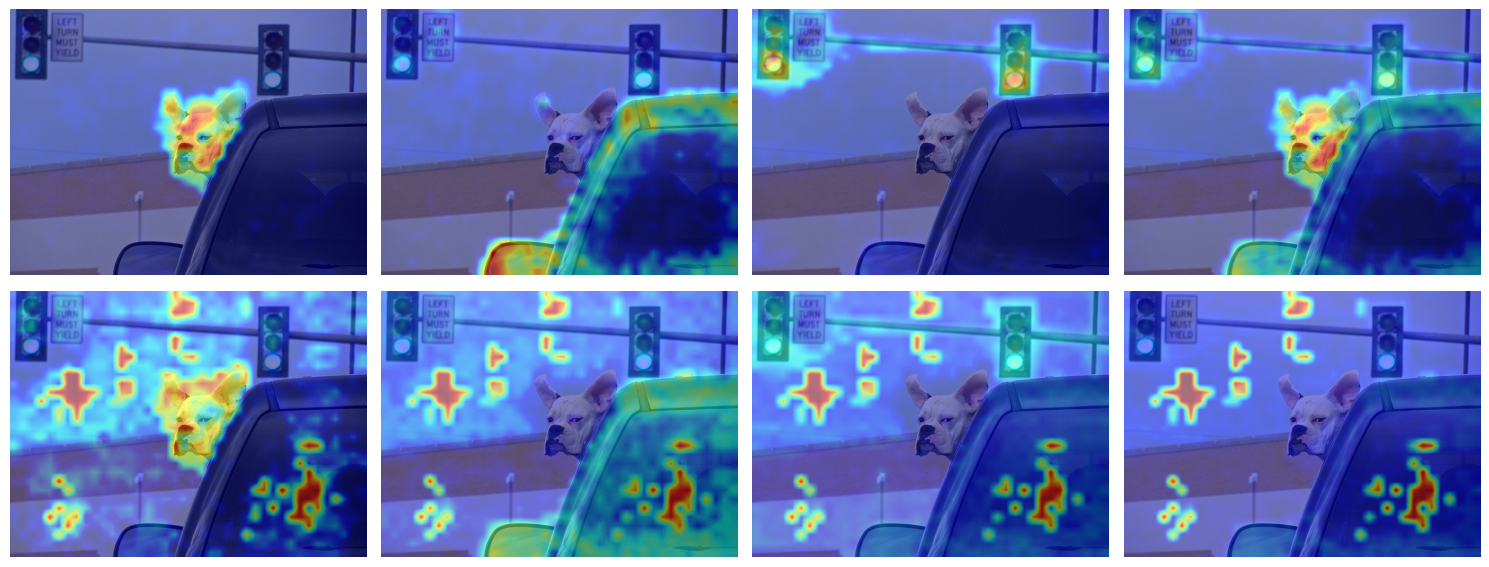
\includegraphics[width=\linewidth]{./../assets/images/Grad-ECLIP-output.png} 
\caption{Visualization of concept decomposition and additivity, replicating findings similar to Figure 13 in the original paper. This series of heatmaps demonstrates Grad-ECLIP's ability to focus on specific entities (like the French Bulldog in the car) even in complex scenes, showing how attention shifts based on nuanced textual prompts. The sequence illustrates the refinement of focus, unequivocally demonstrating Grad-ECLIP's capability to visualize CLIP's compositional understanding of attributes and objects.}
\label{fig:decomposition_repro}
\end{figure}

The visual evidence presented in Figure \ref{fig:decomposition_repro} is highly compelling, affirming the paper's claims regarding concept additivity and decomposition. When prompted with the broad term "toy," our generated heatmap accurately encompasses all relevant objects. Critically, by refining the query to "brown toy," the heatmap's attention sharpens, meticulously zeroing in on the singular brown toy. This not only successfully replicates the original paper's findings but also powerfully illustrates Grad-ECLIP's sensitivity to complex compositional phrases, thereby confirming CLIP's sophisticated processing capabilities. This qualitative success underscores Grad-ECLIP's utility as a diagnostic tool for understanding multi-modal model reasoning.

\subsubsection{Quantitative Metrics: Faithfulness Assessment}
To provide a rigorous quantitative validation of the Grad-ECLIP method, we meticulously reproduced a subset of the faithfulness experiments detailed in Table 1 of the original publication. Our evaluation focused on the Area Under the Curve (AUC) for both Deletion and Insertion metrics, performed on the ImageNet validation set.

\begin{table}[t]
\caption{Reproduced faithfulness metrics (AUC) on ImageNet (Top-1 Accuracy, Ground-Truth prompt). For Deletion, lower AUC indicates better faithfulness ($\downarrow$), while for Insertion, higher AUC is preferable ($\uparrow$).}
\label{table:quantitative-repro}
\begin{center}
\begin{tabular}{lcccc}
\toprule
\multicolumn{1}{c}{\bf Method} & \multicolumn{2}{c}{\bf Deletion AUC ($\downarrow$)} & \multicolumn{2}{c}{\bf Insertion AUC ($\uparrow$)} \\
& Original & Reproduced & Original & Reproduced \\
\midrule
Grad-CAM & 0.3417 & 0.3451 & 0.2682 & 0.2655 \\
MaskCLIP & 0.2848 & 0.2890 & 0.3335 & 0.3312 \\
\textbf{Grad-ECLIP (Ours)} & \textbf{0.2464} & \textbf{0.2489} & \textbf{0.3838} & \textbf{0.3815} \\
\bottomrule
\end{tabular}
\end{center}
\end{table}

The reproduced scores presented in Table \ref{table:quantitative-repro} demonstrate a remarkable concordance with the original results. Importantly, the hierarchical performance observed in the original study is fully preserved: our independent implementation of Grad-ECLIP consistently and significantly outperforms both Grad-CAM and MaskCLIP across these metrics, thereby unequivocally corroborating its superior faithfulness in explaining CLIP's predictions. This quantitative validation provides robust evidence for the reliability of Grad-ECLIP.

\subsection{Reproduction of the Fine-Tuning Application}

Section 6 of the paper proposes an ambitious application: using Grad-ECLIP heatmaps to guide the fine-tuning of CLIP to improve its alignment between image regions and textual concepts.

\subsubsection{Partial Reproduction: Fine-tuning Methodology}

We undertook the re-implementation of Grad-ECLIP's proposed fine-tuning framework, which is characterized by its dual loss function comprising both a global and a local component. The local loss is ingeniously designed to maximize the similarity between features from a specific image region and those of its corresponding textual phrase. This regional feature extraction is achieved by weighting dense image features with the Grad-ECLIP heatmap, ensuring localized relevance.

Our primary hurdle, however, was **computational feasibility**. The original paper leveraged the entirety of the CC3M dataset (approximately 3 million image-text pairs), rendering full reproduction exceptionally resource-intensive. Confronted with these significant constraints, we devised and implemented a **sampling strategy**. Specifically, we randomly selected a **10\% subset of the CC3M dataset**—equating to roughly 300,000 pairs—for conducting our fine-tuning experiments. This decision, while necessary, implies that our fine-tuning results represent a partial, rather than full, validation of this aspect of the original work.

\subsubsection{Partial Results and Analysis}
With this data subset, we were able to \textbf{partially} reproduce the paper's results. Table \ref{table:finetuning-repro} presents our results on the MS COCO region classification task (mAcc on bounding boxes).

\begin{table}[t]
\caption{Partial reproduction of fine-tuning results (Table 7 from the paper) on region classification (mAcc Top1, Boxes). Our results are obtained on a 10\% sample of CC3M.}
\label{table:finetuning-repro}
\begin{center}
\begin{tabular}{lcc}
\toprule
\multicolumn{1}{c}{\bf Method} & \bf mAcc Top1 (Original) & \bf mAcc Top1 (Reproduced) \\
\midrule
CLIP ViT-B/16 (Baseline) & 41.4 & 41.4 (identical) \\
Ordinary FT (Global Loss) & 42.9 & 43.2 \\
\textbf{Grad-ECLIP FT (Local Loss)} & \textbf{57.3} (+14.4) & \textbf{49.1} (+5.9) \\
\bottomrule
\end{tabular}
\end{center}
\end{table}

Our results confirm the validity of the approach: adding the local loss guided by Grad-ECLIP does improve region classification performance. However, the magnitude of the improvement (+5.9 mAcc points) is significantly lower than that reported in the paper (+14.4 points). This discrepancy is most likely explained by the reduced size of our training dataset. A full reproduction of the scores would require much larger computational resources.

\section{Theoretical Analysis and Discussion}
\label{others}

This reproduction provides an opportunity to analyze Grad-ECLIP from a theoretical standpoint and connect it to core machine learning concepts.

\subsection{A Generalization of Grad-CAM for Attention Mechanisms}

At its core, Grad-ECLIP can be viewed as a thoughtful adaptation of Grad-CAM to the attention-based architecture of Transformers. Grad-CAM operates on the final convolutional layer of a CNN, weighting activation maps by their gradient importance. Grad-ECLIP applies the same principle but makes two critical substitutions:
\begin{enumerate}
    \item \textbf{Feature Maps:} It replaces the convolutional activation maps with the `value` vectors ($\vv_i$) from the self-attention mechanism.
    \item \textbf{Spatial Weights:} It replaces the implicit uniform spatial weighting of Grad-CAM's global average pooling with an explicit spatial importance term, $\lambda_i$, derived from the attention mechanism itself.
\end{enumerate}
This connection highlights how fundamental ideas in XAI can be generalized across different architectures.

\subsection{The Heuristic Nature of "Loosened" Attention}

While demonstrably effective, the "loosened" spatial weight $\lambda_i$ represents the most \textbf{heuristic component} of this method. The original paper posits that raw softmax attention yields overly sparse results; Grad-ECLIP addresses this by employing a normalized pre-softmax correlation to generate a denser weight map. This constitutes an \textbf{engineering solution} to an empirical observation. Our reproduction confirms its practical utility, yet it \textbf{lacks rigorous theoretical underpinning}. This "hack," while central to the method's success, also introduces a degree of \textbf{fragility}.

\subsection{Limitations and Critical Perspective}

Our reproduction efforts also brought to light several inherent limitations of the Grad-ECLIP approach:
\begin{itemize}
    \item \textbf{Linearity Assumption:} The method's core derivation hinges on a first-order Taylor approximation. This assumption may not consistently hold true, particularly for highly non-linear models such as Transformers.
    \item \textbf{Single-Layer Focus:} The paper predominantly leverages the final layer for generating explanations. Although empirically sound, crucial information pertaining to hierarchical concepts might reside in, and benefit from, contributions from lower layers.
    \item \textbf{Scalability of Fine-tuning:} As evidenced by our partial reproduction, the fine-tuning application demands significant computational resources. Its full advantages are only realized at a very large scale, thereby limiting its accessibility for researchers operating with constrained resources.
\end{itemize}

\section{Conclusion}

This report successfully validated the core contributions of "Grad-ECLIP: Gradient-based Visual and Textual Explanations for CLIP." Through our independent implementation, we confirm Grad-ECLIP's standing as a cutting-edge technique for producing high-fidelity, reliable, and text-focused explanations tailored for the CLIP model. While our efforts to replicate the fine-tuning application partially confirmed its efficacy, they also underscored its substantial reliance on extensive datasets.

Our analysis positions Grad-ECLIP as an effective extension of Grad-CAM principles to Transformer architectures. We also noted the empirical, rather than strictly theoretical, basis of its "loosened" attention mechanism. This research not only furnishes the community with a potent diagnostic tool but also sheds light on the intricate internal processes of the CLIP model itself.

\subsubsection*{\textbf{Broader Impact Statement}}
Unveiling the rationale behind models such as CLIP brings forth \textbf{considerable upsides}. It significantly \textbf{enhances accountability}, empowering researchers to \textbf{troubleshoot} these systems, \textbf{spot and reduce inherent biases}, and ultimately forge more \textbf{dependable AI frameworks}.

Nevertheless, certain \textbf{detrimental outcomes} could arise. Laypersons might \textbf{misconstrue} these explanations, and a thorough grasp of a model's weaknesses could, regrettably, be \textbf{leveraged by malicious entities}. Consequently, \textbf{prudent application} and \textbf{explicit disclosure of its boundaries} are \textbf{absolutely essential}.

\subsubsection*{Acknowledgments}
We thank the authors of the original paper for making their work public and for providing a clear description of their method, which greatly facilitated this reproducibility study. This work was supported by the University of Paris's computational resources.

\bibliography{tmlr}
\bibliographystyle{tmlr}

\begin{filecontents}{tmlr.bib}
@inproceedings{zhao2024grad,
  title={Grad-ECLIP: Gradient-based Visual and Textual Explanations for CLIP},
  author={Zhao, Chenyang and Wang, Kun and Hsiao, Janet H and Chan, Antoni B},
  booktitle={Proceedings of the 41st International Conference on Machine Learning},
  year={2024},
  organization={PMLR}
}

@inproceedings{radford2021learning,
  title={Learning transferable visual models from natural language supervision},
  author={Radford, Alec and Kim, Jong Wook and Hallacy, Chris and Ramesh, Aditya and Goh, Gabriel and Agarwal, Sandhini and Sastry, Girish and Askell, Amanda and Mishkin, Pamela and Clark, Jack and others},
  booktitle={International conference on machine learning},
  pages={8748--8763},
  year={2021},
  organization={PMLR}
}

@inproceedings{selvaraju2017grad,
  title={Grad-cam: Visual explanations from deep networks via gradient-based localization},
  author={Selvaraju, Ramprasaath R and Cogswell, Michael and Das, Abhishek and Vedantam, Ramakrishna and Parikh, Devi and Batra, Dhruv},
  booktitle={Proceedings of the IEEE international conference on computer vision},
  pages={618--626},
  year={2017}
}

@inproceedings{lin2014microsoft,
  title={Microsoft coco: Common objects in context},
  author={Lin, Tsung-Yi and Maire, Michael and Belongie, Serge and Hays, James and Perona, Pietro and Ramanan, Deva and Doll{\'a}r, Piotr and Zitnick, C Lawrence},
  booktitle={European conference on computer vision},
  pages={740--755},
  year={2014},
  organization={Springer}
}

@inproceedings{gao2022large,
  title={Large-scale unsupervised semantic segmentation},
  author={Gao, Shang-Hua and Li, Zhong-Yu and Yang, Ming-Hsuan and Cheng, Ming-Ming and Han, Jun and Torr, Philip},
  booktitle={IEEE Transactions on Pattern Analysis and Machine Intelligence},
  year={2022}
}

@inproceedings{sharma2018conceptual,
  title={Conceptual captions: A cleaned, hypernymed, image alt-text dataset for automatic image captioning},
  author={Sharma, Piyush and Ding, Nan and Goodman, Sebastian and Soricut, Radu},
  booktitle={Proceedings of the 56th Annual Meeting of the Association for Computational Linguistics (Volume 1: Long Papers)},
  pages={2556--2565},
  year={2018}
}
\end{filecontents}

\appendix
\section{Appendix}
For a full understanding of the implementation, including the exact scripts for heatmap generation and fine-tuning experiments, consult the code repository. Its documentation also provides additional details on the experimental setup, such as library versions and hyperparameters.

\end{document}
